\section{Algorithm Details}
\label{sec:algo_details}

\subsection{Spectral Radius Scale}
\label{sec:spectral_radius}

Given the target spectral radius
\[
R = \Theta\left(\sqrt{d_{\text{out}}/d_{\text{in}}}\right)
  = c \left(\sqrt{d_{\text{out}}/d_{\text{in}}}\right),
\]
the constant \(c\) serves as a scalar that sets the branch output magnitude
relative to the residual stream. By tuning \(c\), one can precisely control
the signal-to-noise ratio along the deep residual path, balancing the
contributions of the Attention/FFN blocks against the skip connection.
Properly choosing \(c\) is therefore essential for stabilizing depth-wise
signal propagation in Transformers.


\begin{figure}[ht]
    \centering
    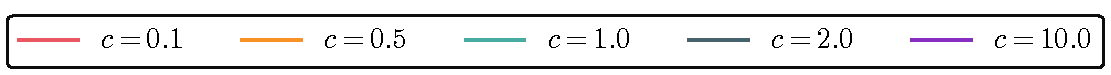
\includegraphics[width=0.7\linewidth]{figures/details/radius_legend.pdf}
    \begin{subfigure}{0.32\linewidth}
        \centering
        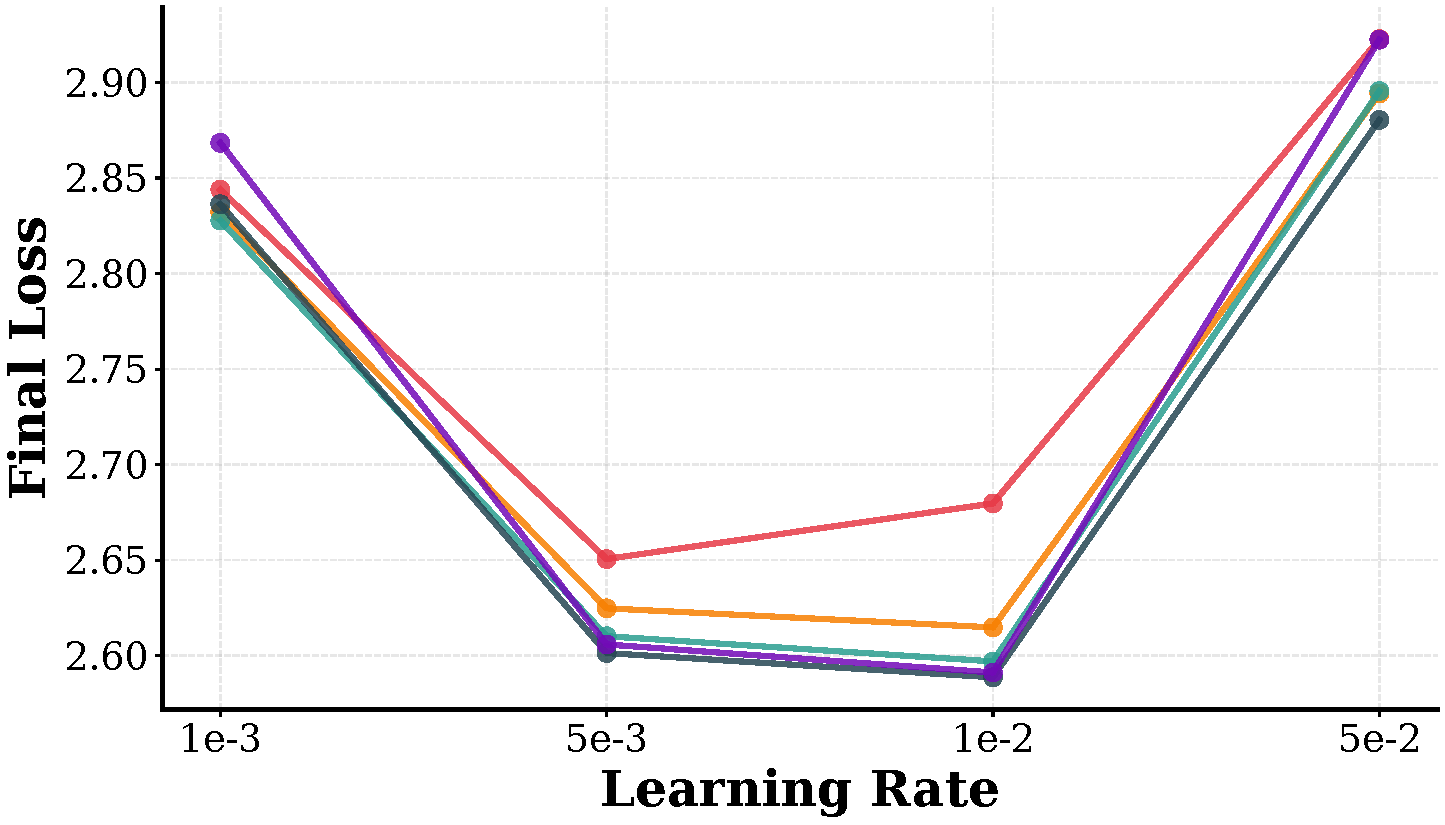
\includegraphics[width=\linewidth]{figures/details/radius_search.pdf}
        \caption{Radius scale search.}
        \label{fig:radius_search}
    \end{subfigure}
    \hfill
    \begin{subfigure}{0.32\linewidth}
        \centering
        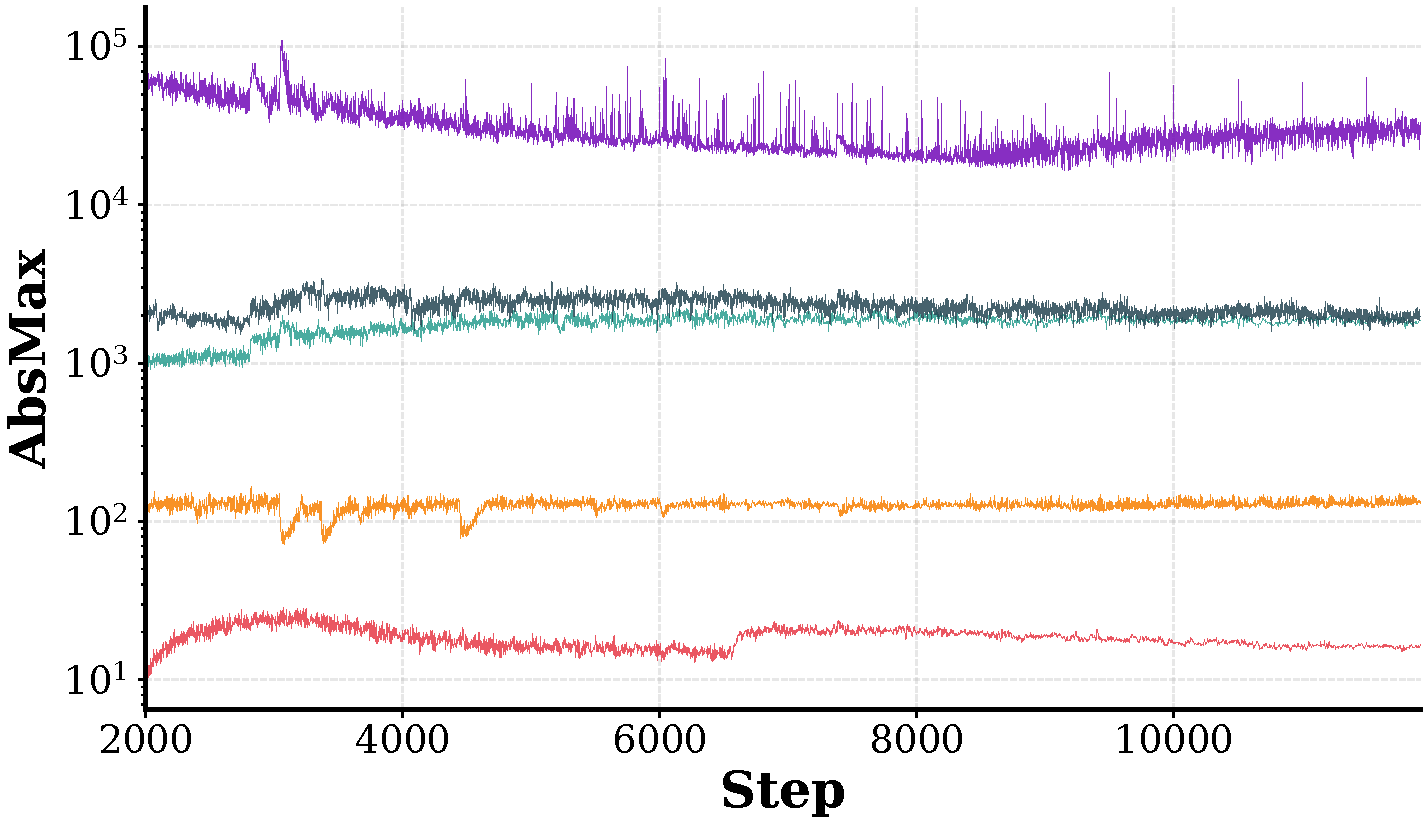
\includegraphics[width=\linewidth]{figures/details/radius_mlp_absmax.pdf}
        \caption{\texttt{AbsMax} of FFN activations.}
        \label{fig:radius_mlp_absmax}
    \end{subfigure}
    \hfill
    \begin{subfigure}{0.32\linewidth}
        \centering
        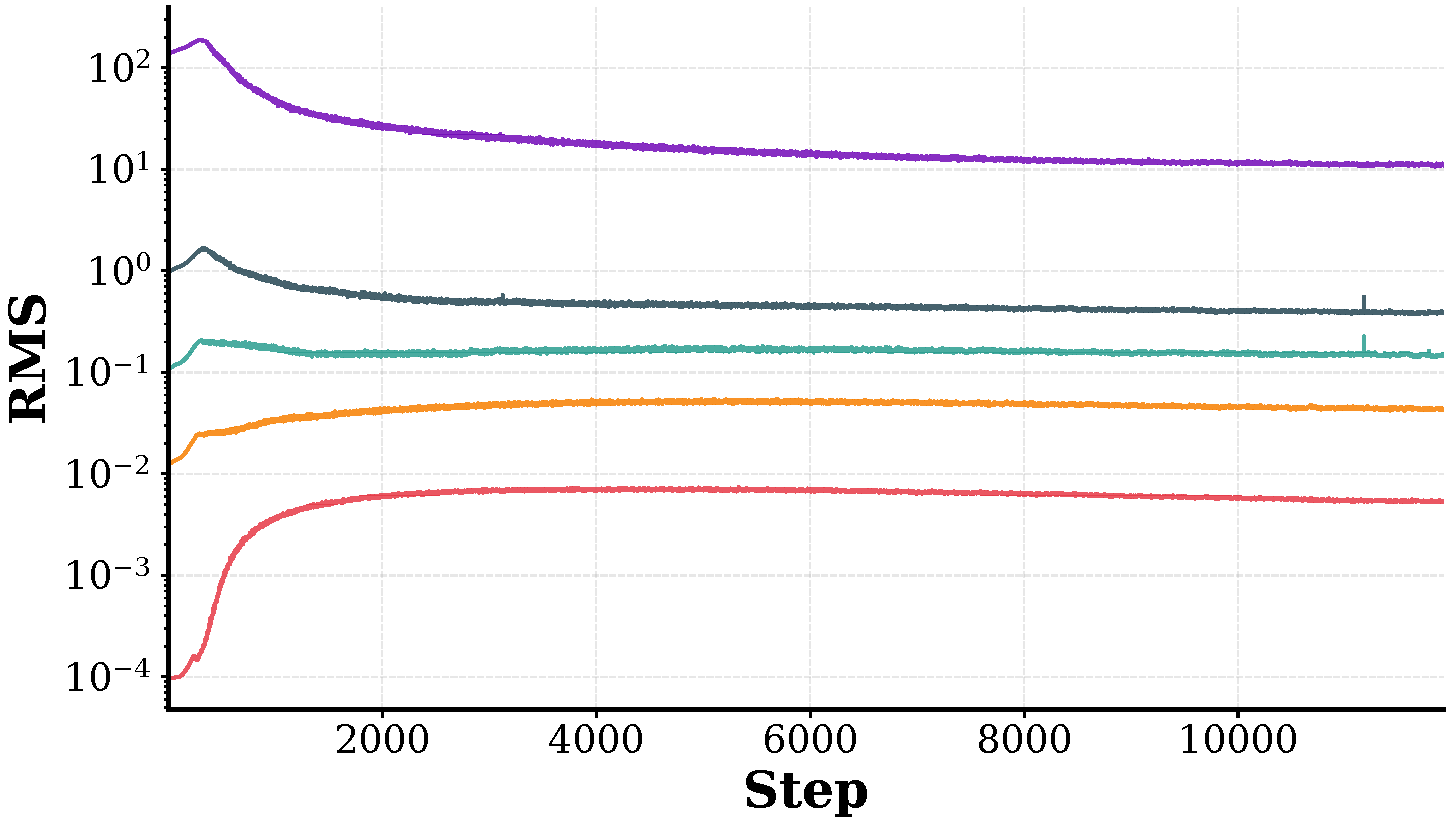
\includegraphics[width=\linewidth]{figures/details/radius_mlp_rms.pdf}
        \caption{\texttt{RMS} of FFN activations.}
        \label{fig:radius_mlp_rms}
    \end{subfigure}
    \caption{\textbf{Ablation of radius scaling on \textit{optimization} and \textit{activation}.}
    (a) Final loss vs. learning rate for varying radius scales $c$. A moderate scale (e.g. $c=2.0$) achieves the best performance.
    (b) AbsMax and (c) RMS of FFN activations during training. AbsMax monotonically follows the radius scale, whereas RMS follows a clear power-law scaling with $c$.
    }
    \label{fig:radius_all}
\end{figure}

\subsection{Learning Rate Scaler}
\label{sec:lr_scaler}

We propose a unified view in which each learning rate scaler enforces a consistent \textbf{effective step size} under a chosen \textbf{norm metric} and \textbf{initialization scheme}.

In the update rule $\mW \gets \mW - \eta R \mPhi$, $R$ scales the update size. To avoid instability caused by heterogeneous layer shapes, we select $R$ to maintain a constant \emph{effective step size}~---~defined as the ratio of update-to-weight magnitude under a norm metric $\|\!\cdot\!\|$ :
\begin{equation}
    \frac{\|\Delta \mW\|}{\|\mW\|} = \frac{\|\eta R \mPhi\|}{\|\mW\|} \approx \eta.
\end{equation}


We evaluate three common learning rate scalers below:
\begin{equation}
    R =
\begin{cases}
\sqrt{d_{\mathrm{out}}/d_{\mathrm{in}}},
    & \text{(\textit{Spectral $\boldsymbol{\mu}$P Scaler)}} \\[6pt]
 \sqrt{\max(d_{\mathrm{out}}, d_{\mathrm{in}})} \cdot 0.2 ,
    & \text{(\textit{Align-Adam-RMS Scaler})} \\[6pt]
\sqrt{\max(1, d_{\mathrm{out}}/d_{\mathrm{in}})},
    & \text{(\textit{Spectral Kaiming Scaler})}
\end{cases}
\label{eq:lrscaler}
\end{equation}


\begin{figure}[ht]
    \centering
    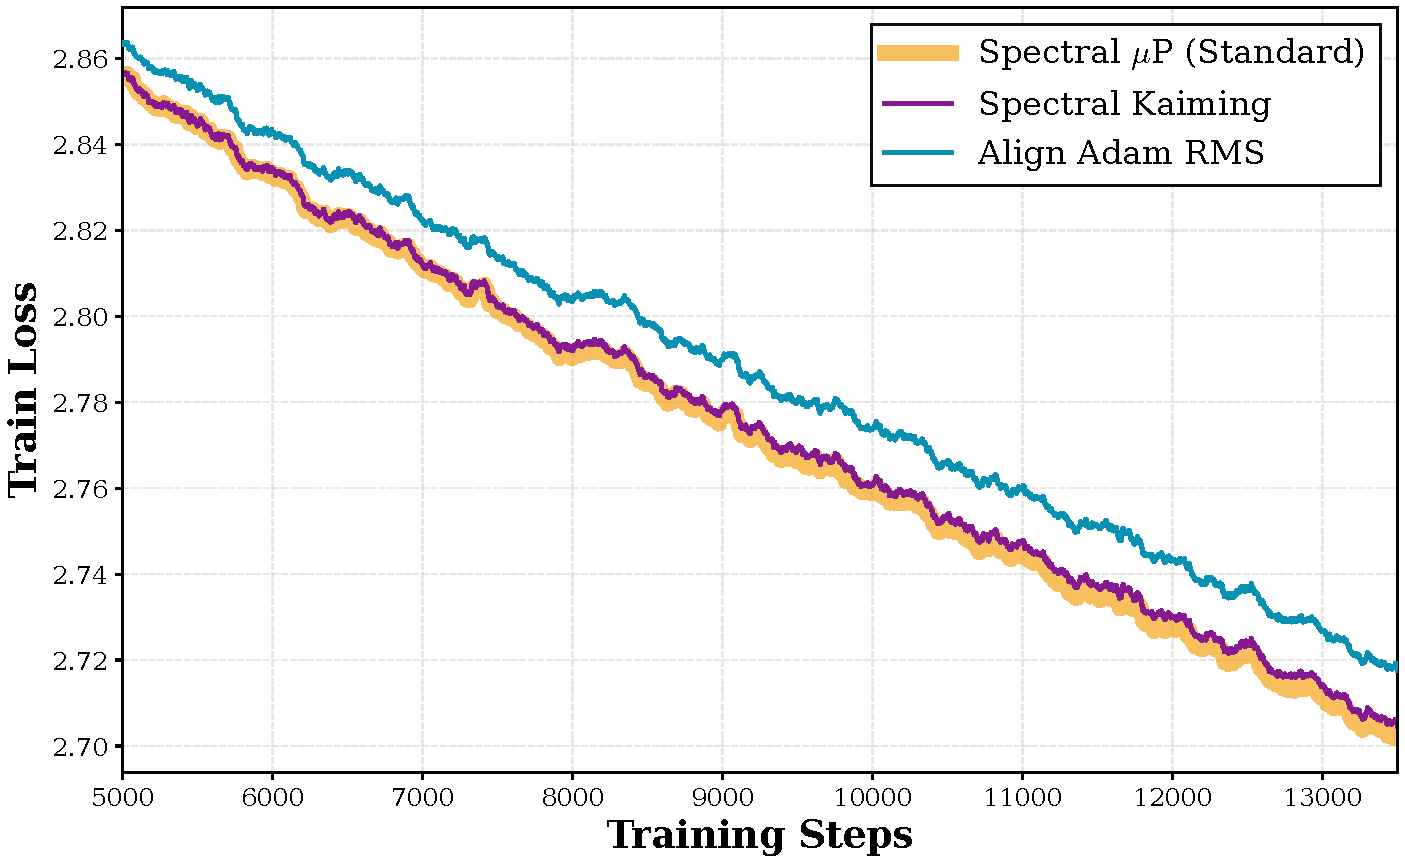
\includegraphics[width=0.5\linewidth]{figures/details/lrscaler_ablation_loss.pdf}
    \caption{
    \textbf{Ablation of learning rate scalers.} Each curve represents the optimal validation loss obtained via a learning rate grid search. \textbf{Spectral $\boldsymbol{\mu}$P} (yellow) outperforms \textbf{Align-Adam-RMS} (blue), validating the optimality of $\boldsymbol{\mu}$P-aligned scaling under the Spectral $\boldsymbol{\mu}$P condition.
    }
    \label{fig:lr_scaler}
\end{figure}

\begin{itemize}[leftmargin=*]

    \item \textbf{Spectral $\boldsymbol{\mu}$P Scaler.}
    Enforces the \emph{RMS-to-RMS operator norm} invariance from~\cref{sec:bg_mup}.
    It ensures that both $\mW$ and $\Delta\mW$ satisfy the $\boldsymbol{\mu}$P scaling $\|\mW\|_2=\Theta(\sqrt{d_{\mathrm{out}}/d_{\mathrm{in}}})$,
    forming the geometric basis of our Spectral Sphere Optimizer.

    \item \textbf{Align-Adam-RMS Scaler.}
    A heuristic for consistent relative learning rates in the \emph{RMS norm}
    under fixed standard-deviation initialization.
    Empirically, it aligns per-layer update RMSnorm to AdamW,
    enabling direct transfer of AdamW-tuned hyperparameters
    (e.g. learning rate, weight decay)
    to the spectral method~\citep{liu2025muonscalablellmtraining}.

    \item \textbf{Spectral Kaiming Scaler.}
    Targets the \emph{spectral norm} under Kaiming initialization
    ($\mW \sim \mathcal{N}(0, 1/d_{\mathrm{in}})$)~\citep{He2015Initialization}.
    Random matrix theory establishes that such matrices satisfy
    $\|\mW\|_2 \approx 1 + \sqrt{d_{\mathrm{out}}/d_{\mathrm{in}}}$.
    This scaling prevents vanishing pre-activations in bottleneck layers
    where $d_{\mathrm{out}} \ll d_{\mathrm{in}}$~\citep{pethick2025trainingdeeplearningmodels}.

\end{itemize}

Experimental results (\cref{fig:lr_scaler}) favor the \textbf{Spectral $\boldsymbol{\mu}$P} scaler, supporting the theoretical scaling condition in~\cref{sec:bg_mup}. This demonstrates that \emph{optimizing on a spectral manifold requires a scaler explicitly calibrated to the spectral norm.}


\subsection{Module Granularity }
\label{sec:module_gran}
\begin{figure}[ht]
    \centering
    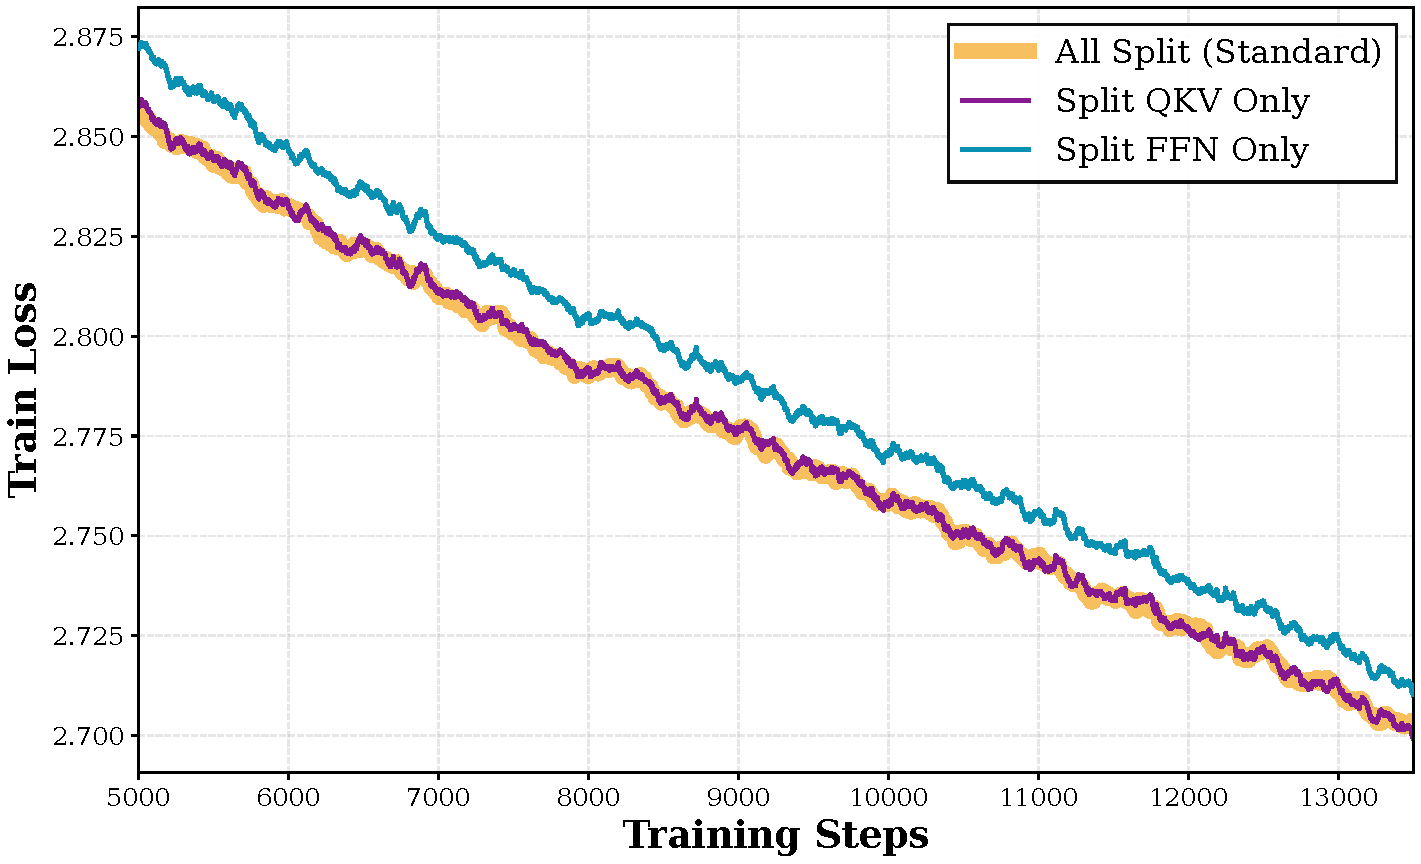
\includegraphics[width=0.5\linewidth]{figures/details/module_ablation_loss.pdf}
    \caption{
    \textbf{Ablation of module granularity for \emph{initialization} and \emph{optimization}.}
    Splitting QKV per head alone yields the most significant performance gain.
    Although splitting the FFN gate/up weights produces nearly the same loss curve as no-split, we maintain this split to respect their distinct functional roles; the overlapping curve is omitted from the figure.
    }
    \label{fig:granularity}
\end{figure}
To maximize computational efficiency, modern Transformer implementations such as Megatron-LM~\citep{megatron-lm} fuse several matrices into a single physical tensor (e.g. the QKV projections or the SwiGLU gate/up matrices).
However, since these modules have distinct functional roles, imposing a unified constraint on the fused tensor is suboptimal as shown in~\cref{fig:granularity}.
Instead, we decompose fused tensors and treat each submatrix as an independent module.
We apply \textbf{per module spectral initialization and optimization} at this finer granularity by default (e.g. splitting attention QKV per head and separating FFN gate/up). Note that granularity is tunable depending on infra speed.

Under our spectral $\boldsymbol{\mu}$P initialization scheme (also discussed in~\cref{sec:lr_scaler}), the weight matrix is constructed by first sampling
$\mW_k \sim \mathcal{N}(0,\sigma^2)$ and subsequently projecting it onto the spectral sphere:
\[
\mW =
c \sqrt{\frac{d_{\mathrm{out}}}{d_{\mathrm{in}}}}
\cdot
\frac{\mW_k}{\|\mW_k\|_2}.
\]
